\documentclass[12pt, a4paper]{article}

% ******************************** PACKAGE ****************************
\usepackage[top=1.5cm, bottom=1.5cm, left=1.5cm, right=1.5cm]{geometry}
\usepackage{amsmath}
\usepackage{amsmath}
\usepackage{amssymb}
\usepackage{enumitem}
\usepackage{fancyhdr}
\pagestyle{fancy}
\usepackage{tikz}
\usepackage{adjustbox}
\usepackage[colorlinks=true]{hyperref}
\usepackage{lastpage}

% ******************************** SETUP ********************************
\newcommand{\disablelinkcolor}{%
	\hypersetup{linkcolor=black}%
}
\newcommand{\enablelinkcolor}{
	\hypersetup{
		linkcolor=blue
	}
}

\pagestyle{fancy}
\fancyhf{}
\fancyhead[L]{\nouppercase{\leftmark}}
\fancyhead[R]{page \thepage\ of \pageref*{LastPage}}
\fancyfoot[R]{\textit{\textbf{Andrea Savastano}}}

% *************************** MAIN PAGE INFO *****************************
\title{Prestazioni CDMA}
\author{Andrea Savastano}
\date{\today}

% ******************************** DOCUMENTO ****************************
\begin{document}
	\disablelinkcolor	
	\maketitle
	\thispagestyle{empty}
	\tableofcontents
	
	\newpage
	\section{Calcolo teorico media e varianza}
	\begin{itemize}[itemsep=0pt]
	\item $N$: numero di utenti
	\item $\mathcal{E}_s$: Energia del segnale trasmesso $s$ 
	\item $s_1$: segnale aspettato 
	\item $c_n$: chirping code dell'utente \textit{n}-esimo
	\item $L_c$: lunghezza del chirping code
\end{itemize}

\[
s_1 = \mathcal{E}_s \pm \sum_{k=1}^{L_c}\left(\sum_{n=2}^{N}c_{1k}\cdot c_{nk}\right)
= \mathcal{E}_s \pm \sum_{k=1}^{L_c}X_k
\] 

\begin{itemize}[itemsep=0pt]
	\item $\{X_k\}_{k=1,\dots,L_c}$: variabili aleatorie indipendenti
\end{itemize}
\hrule

\subsection{Calcolo di $\mathrm{E}[X_k]$ e $\mathrm{VAR}[X_k]$}
\[
\Bigg( c_{nk}\in [-1,1] \Bigg) \implies \Bigg( \mathrm{E}[c_{nk}] = 0 \Bigg)
\] \\\vspace{-.5cm} \[
\mathrm{\mathrm{E}}[X_k] = \mathrm{E}\left[\sum_{n=2}^{N}c_{1k}\cdot c_{nk}\right] 
= c_{1k}\cdot \mathrm{E}\left[\sum_{n=2}^{N}c_{nk}\right]
= c_{1k}\cdot \sum_{n=2}^{N}\mathrm{E}[c_{nk}] 
= 0
\] \\\vspace{-.5cm} \[
\mathrm{VAR}[X_k] = \mathrm{E}[X_k^2] - \mathrm{E}^2[X_k] = \mathrm{E}[X_k^2] = \mathrm{E}\left[\left(\sum_{n=2}^{N}c_{1k}\cdot c_{nk}\right)^2\right] =
\mathrm{E}\left[ c_{1k}^2\cdot \sum_{n=2}^{N}c_{nk}^2 \right] =
\mathrm{E}\left[ \sum_{n=2}^{N}1 \right] =
N-1
\]
\hrule

\subsection{Calcolo di $\mathrm{E}[n]$ e $\mathrm{VAR}[n]$}
\[
\mathrm{E}[n] = \mathrm{E}\left[ \sum_{k=1}^{L_c}X_k \right] =
\sum_{k=1}^{L_c}\mathrm{E}\left[ X_k \right] = \sum_{k=1}^{L_c}0 = 0
\] \\\vspace{-1.3cm} 

\[
\Bigg( \{X_k\}_{k=1,\dots,L_c}	\text{indipendenti} \Bigg) \implies \Bigg(
\mathrm{VAR}[X_1+X_2+\dots+X_{Lc}] = \mathrm{VAR}[X_1]+\mathrm{VAR}[X_2]+\dots+\mathrm{VAR}[X_{Lc}] \Bigg)
\] \\\vspace{-1.2cm} 

\[
\implies \mathrm{VAR}[n] = \mathrm{VAR}\left[ \sum_{k=1}^{L_c}X_k \right] =
\sum_{k=1}^{L_c}\mathrm{VAR}\left[ X_k \right] = 
\sum_{k=1}^{L_c}\left( N-1 \right) = 
L_c \cdot (N-1)
\] \\
Applicando il \textit{Teorema Centrale del Limite},\\
essendo $\{X_k\}_{k=1,\dots,L_c}$
indipendenti con $\mathrm{E}[X_k]=0$ e $\mathrm{VAR}[X_k]=(N-1)$ la loro somma genera una variabile aleatoria $n$ con distribuzione Gaussiana e questa è il rumore che si aggiunge in ricezione.
\[
\sum_{k=1}^{L_c}X_k = n, \quad\boxed{ n\sim\mathcal{N}\Big(0,\, L_c(N-1)\Big) }
\implies \Bigg( s_1 = \mathcal{E}_s \pm \sum_{k=1}^{L_c}X_k = \mathcal{E}_s \pm n \Bigg)
\]
	
	\newpage
	\section{Grafici}
	\subsection{Distribuzione somma di \(X_k\)}
	\begin{adjustbox}{width=.95\paperwidth, center}
	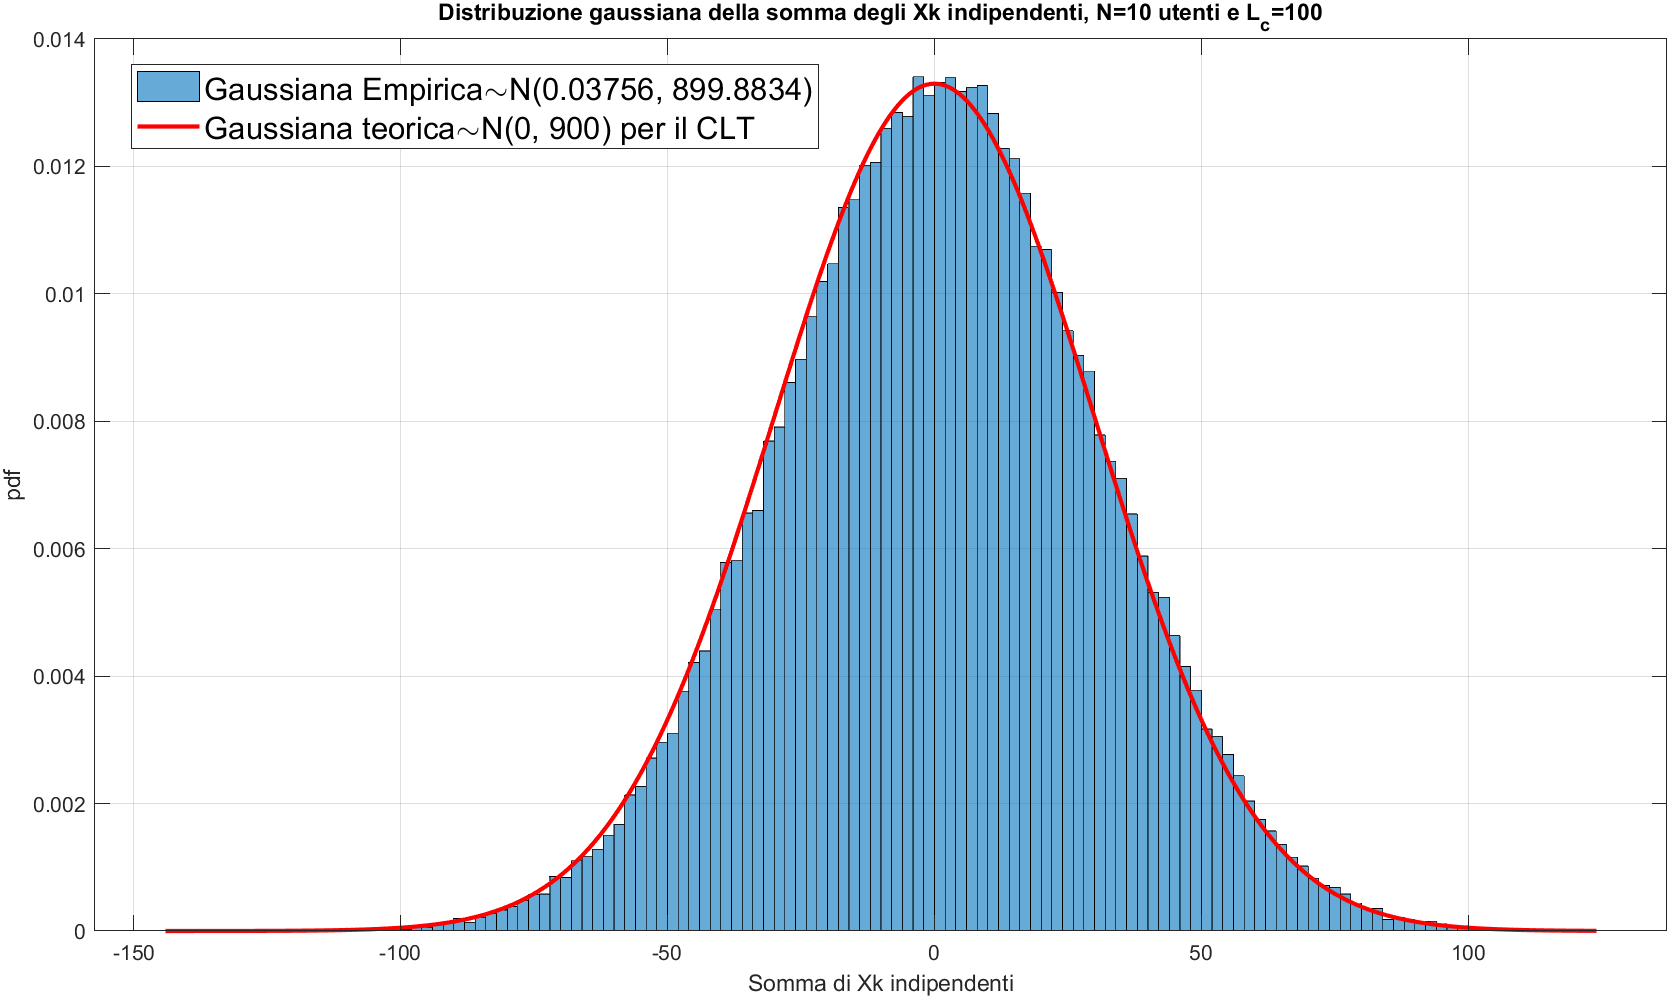
\includegraphics{images/distribuzioneGaussianaEmpTh.png}
\end{adjustbox}\\\\
Svolgendo l'esperimento \( \sum_{k=1}^{L_c}\left(\sum_{n=2}^{N}c_{1k}\cdot c_{nk}\right)
= \sum_{k=1}^{L_c}X_k \) con \(N=10\) utenti e \(L_c=100\) lunghezza del chirping code per ogni utente, si dimostra empiricamente che la somma degli \(X_k\) indipendenti \( \sum_{k=1}^{L_c}X_k = n \) ha una distriuzione gaussiana (di colore blu nel grafico) che segue quella teorica (di colore rosso nel grafico), con media \(0.038 \to 0\) e varianza \(899.883 \to 900=L_c(N-1)\), come era stato dimostrato teoricamente nella pagina precedente.
	
	\newpage
	\subsection{Prestazioni CDMA al variare di \(SNR_{dB}\)}
	\begin{adjustbox}{width=.95\paperwidth, center}
	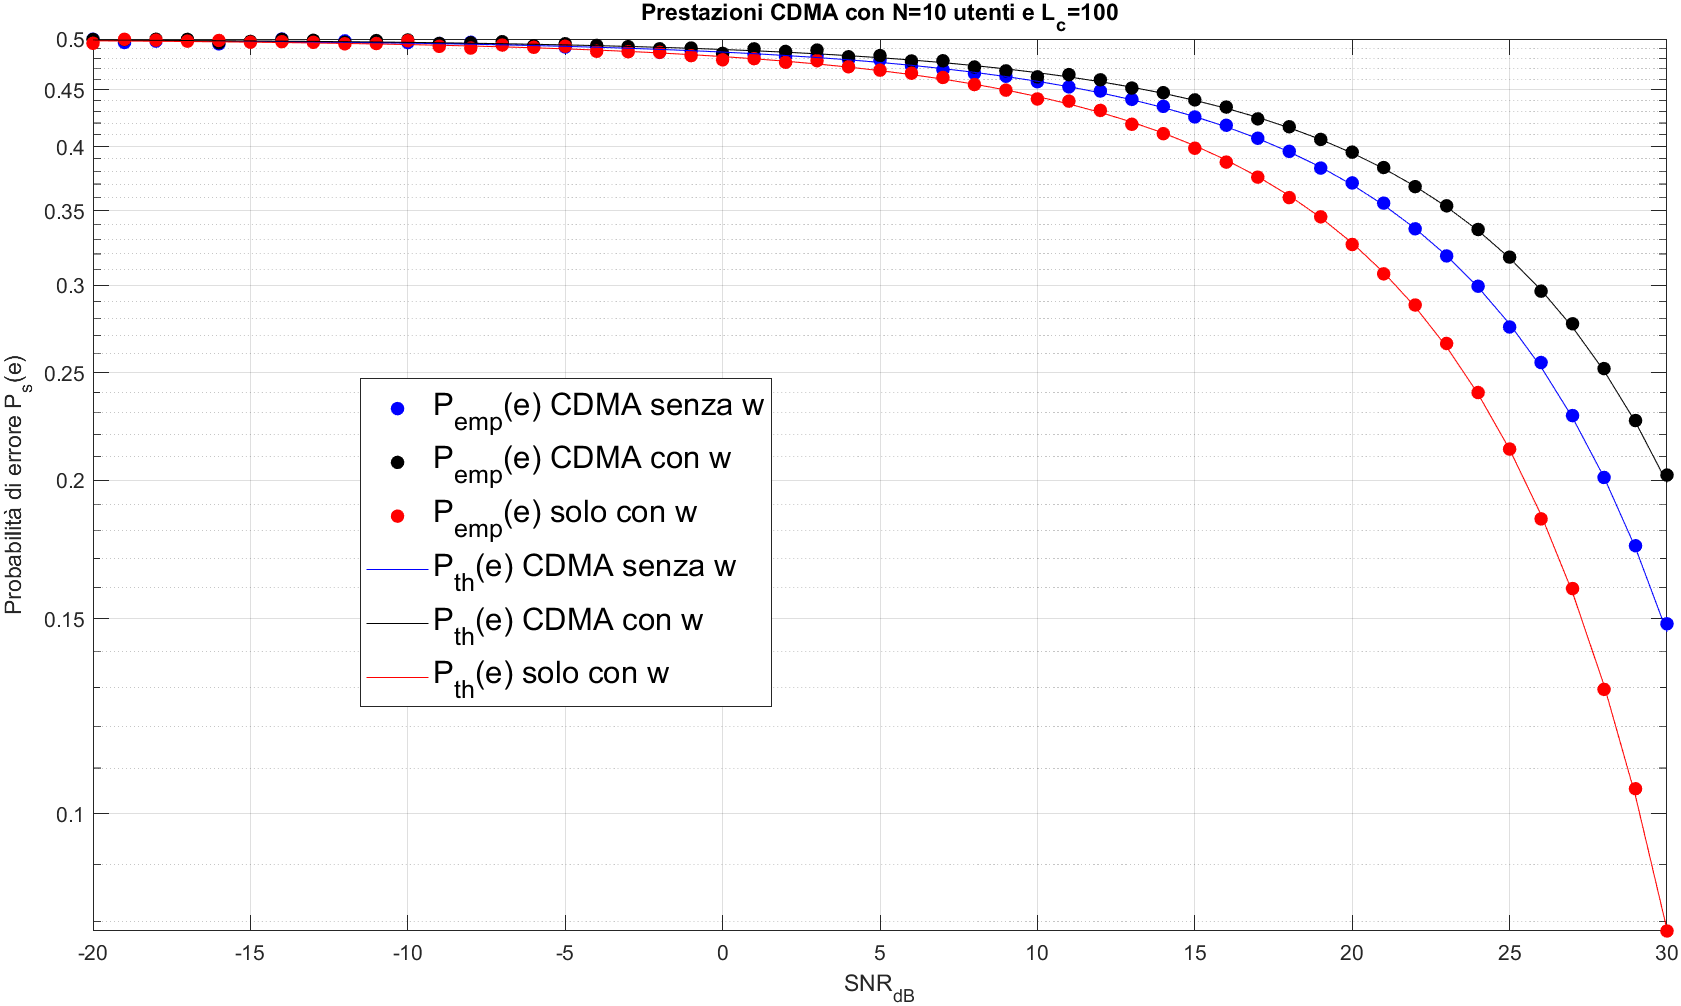
\includegraphics{images/prestazioniCDMA1.png}
\end{adjustbox}\\\\
Simulando la trasmissione CDMA con \(N=10\) e \(L_c=100\) sono state ricavate le tre \(P_{emp}(e)\) e le rispettive \(P_{th}(e)\) che seguono lo stesso andamento.\vspace{.3cm}\\
La \(P_{emp}(e)\) blu rappresenta le prestazioni della trasmissione CDMA senza rumore \(w\) aggiuntivo, considerando quindi \(s_1 = \mathcal{E}_s \pm n, \; n\sim\mathcal{N}(0,\,L_c(N-1))\).\vspace{.3cm}\\
La \(P_{emp}(e)\) nera rappresenta le prestazioni della trasmissione CDMA con rumore \(w\) aggiuntivo,\\
considerando quindi \(s_1 = \mathcal{E}_s \pm n + w, \; w\sim\mathcal{N}(0,\,\frac{N_0}{2})\).\vspace{.3cm}\\
La \(P_{emp}(e)\) rossa rappresenta le prestazioni della trasmissione con solo rumore \(w\),\\ considerando quindi \(s_1 = \mathcal{E}_s + w\).\vspace{.3cm}\\
Si nota dal grafico che la \(P(e)\) nera decade più lentamente rispetto alle altre al crescere di \(SNR_{dB}\) e denota quindi le prestazioni peggiori.\\
In questa simulazione è stato scelto \(N_0\) di \(w\) tale da non influire eccessivamente nella trasmissione per ottenere tre andamenti distinti. Infatti se si aumentasse \(N_0\), la \(P(e)\) nera si sovrapporrebbe con la \(P(e)\) rossa perchè il rumore \(n\) risulterebbe trascurabile rispetto a \(w\), mentre la \(P(e)\) blu denoterebbe le prestazioni migliori.
	
	\newpage
	\subsection{Prestazioni CDMA al variare di \(N\)}
	\begin{adjustbox}{width=.95\paperwidth, center}
	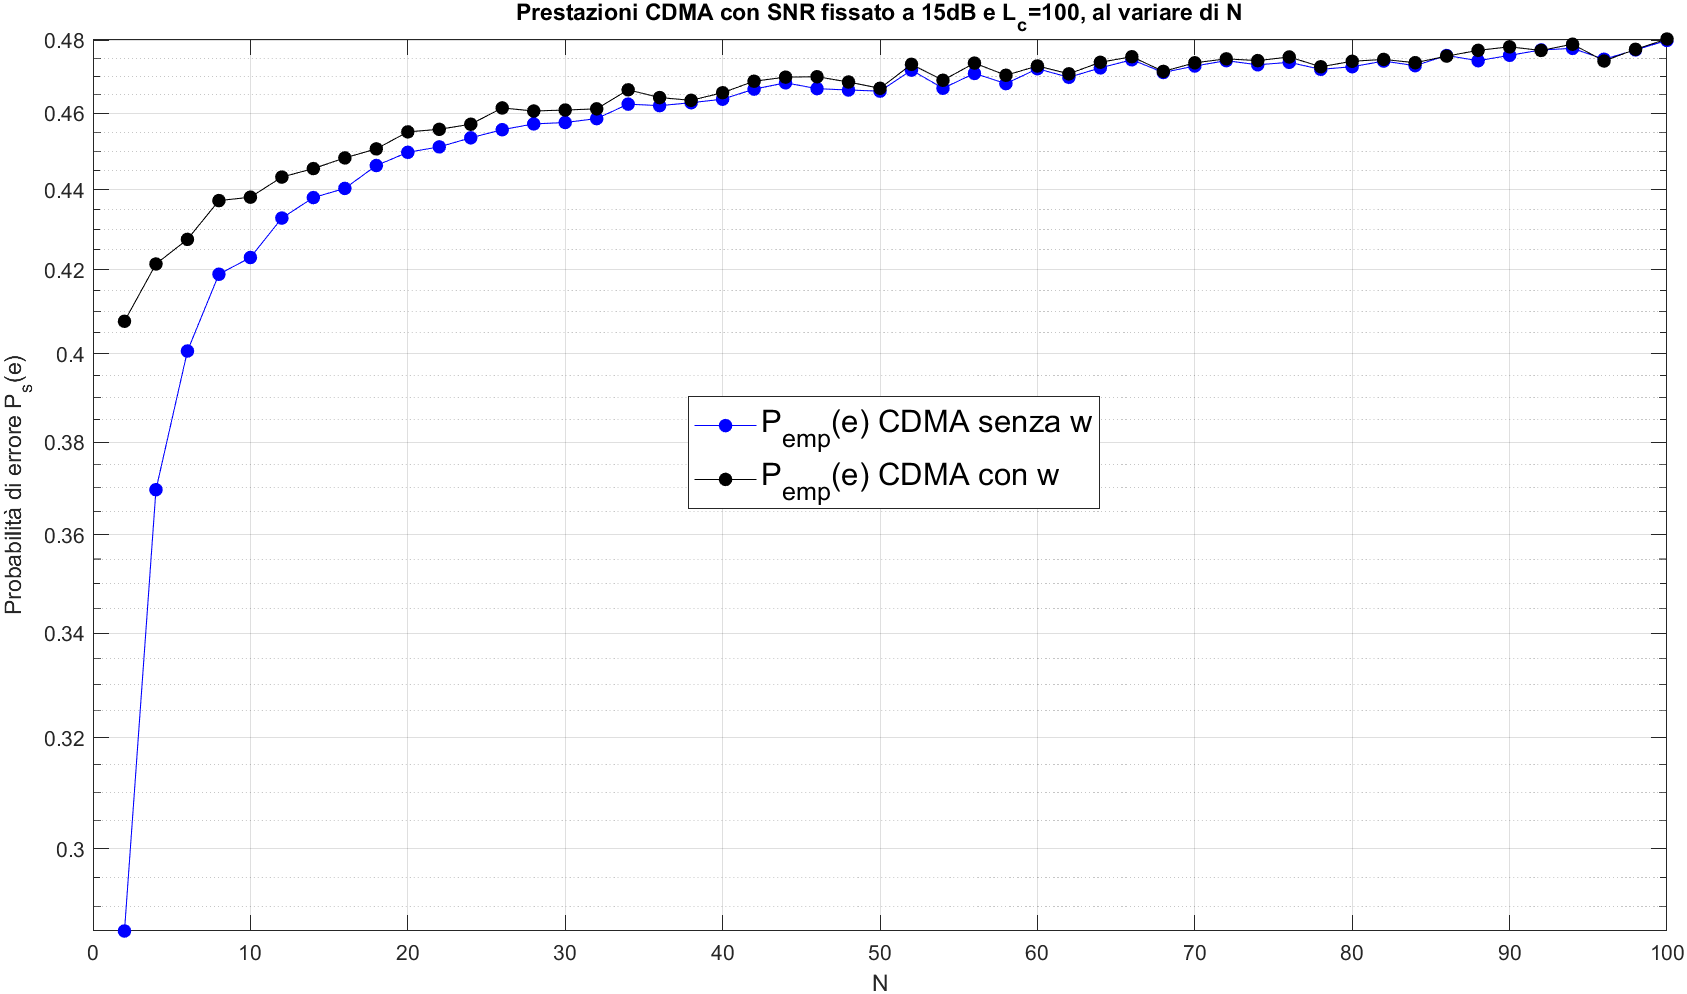
\includegraphics{images/prestazioniCDMA2.png}
\end{adjustbox}\\\\
In questa seconda simulazione è stato scelto di fissare l'\(SNR_{dB}\) a \(15\,dB\) ed \(L_c\) a \(100\) e valutare le prestazioni al variare di \(N\in[2,100]\).\vspace{.3cm}\\
Entrambe le \(P_{emp}(e)\) crescono all'aumentare di \(N\) perchè aumenta sempre più la varianza del rumore \(n\) che dipende da \(L_c\) ed \(N\), infatti \(n\sim\mathcal{N}(0,\,L_c(N-1))\).\\
Per \(N\) piccoli, quindi per \(N\in[2,30]\), si nota una maggiore differenza tra la \(P_{emp}(e)\) senza \(w\) aggiuntivo e quella con \(w\), infatti quest'ultima denota prestazioni peggiori.\\
Invece al crescere di \(N\), quindi per \(N>30\), la varianza del rumore \(n\) aumenta sempre di più per entrambe le \(P_{emp}(e)\) fino a far diventare trascurabile \(w\) rispetto ad \(n\) per la \(P_{emp}(e)\) nera, facendo sovrapporre i due grafici.
	
\end{document}